\documentclass[10pt, final]{article}

\usepackage{cite}
\usepackage{fullpage}
\usepackage{graphicx}
\usepackage{hyperref}
\usepackage{amsmath,float}
\usepackage{subcaption}
\usepackage{url}
\usepackage[ruled,vlined,commentsnumbered,titlenotnumbered,norelsize]{algorithm2e}
\usepackage{geometry}
\geometry{
	a4paper,
	total={170mm,257mm},
	left=20mm,
	top=20mm,
}

% Line break with additional spacing. Default is .75 line-height extra spacing
% Extra space is put in to allow line breaks immediately after \item
\newcommand{\br}[1][.75]{\ \\[#1\baselineskip]}

\parindent 0pt

\begin{document}
	\begin{center}
		\LARGE{\textbf{AI in Game Playing: Sokoban Solver}}\\
		\Large{\textbf{CS 221 Project Progress Report}}\\
		\Large{Anand Venkatesan, Atishay Jain, Rakesh Grewal }
	\end{center}
	
	\section{Introduction}
	Sokoban is a very popular transportation puzzle game that is played extensively with its variants. Solving Sokoban is a well acknowledged area of research because it exist as a NP-Hard problem and PSPACE-Complete. The high level strategies, complicated techniques and high branching factor of this game makes it difficult to solve. The goal of our project is to develop an AI agent that can play the game effectively. In this progress report, we delve deeper into the ideas furnished in our proposal by (1) pointing out the game mechanics in a straightforward manner (2) describing the states and explaining how it is modeled in our algorithms (3) detailing our algorithms to calculate the best moves for the levels of the game (4) defining proper pruning techniques that are implemented to ameliorate the performance of the algorithm (5) providing results and comparing the developed algorithm using standard metrics of evaluation. We conclude with the next steps we plan to take up to finish this project.
	
	\section{General Game Mechanics}
	The rigorous rules and the confined space of the game is described exhaustively in the Section $2$ (\textit{Task Definition}) of our proposal. To briefly define the game play in simple terminology, we can say that the goal of this game if to move the crates to proper storage locations by moving in a constricted space provided in each level. The player fails to complete the game if he gets locked up in positions where the player is not able to move himself or the crates further. This game play is shown in Fig.1 \br
	\begin{figure}[h!]
		\centering
		{
			\begin{subfigure}[h!]{1.7in}
				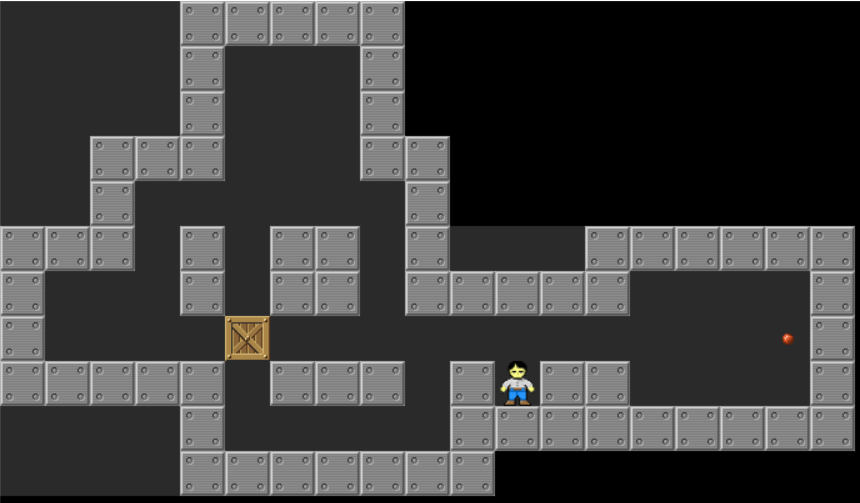
\includegraphics[height=1in]{pic1.png}
			\end{subfigure}
			~$\mathbf{\Longrightarrow}$~
			\begin{subfigure}[h!]{1.7in}
				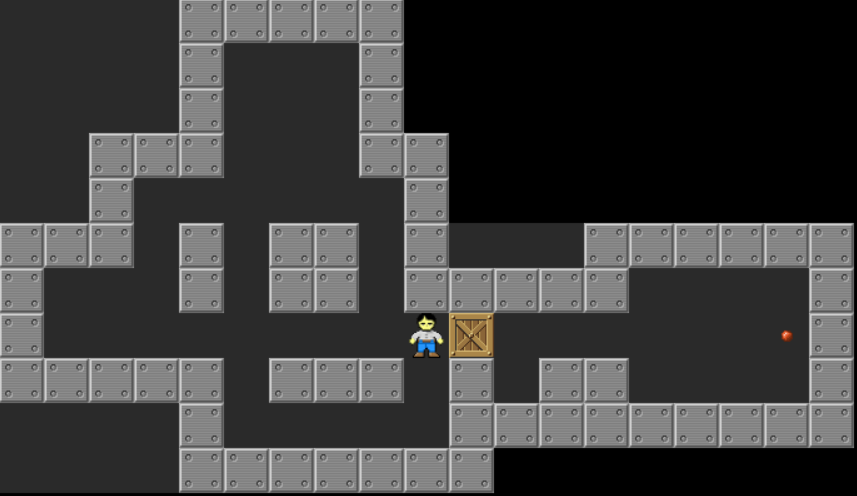
\includegraphics[height=1in]{pic2.png}
			\end{subfigure}
			~$\mathbf{\Longrightarrow}$~
			\begin{subfigure}[h!]{1.7in}
				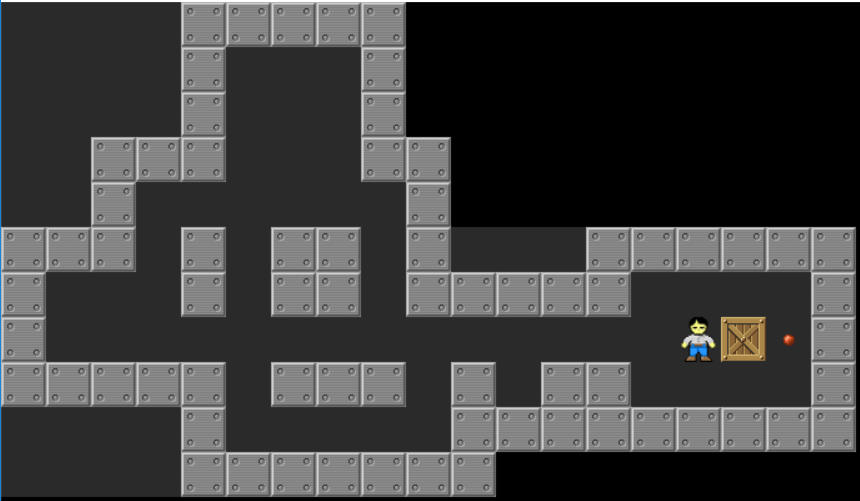
\includegraphics[height=1in]{pic3.png}
		\end{subfigure}}
		\caption{Game play of Sokoban}
		\label{fig:chain}
	\end{figure}
	\section{States and Modeling}
	The game of sokoban can alternatively be considered as a search problem where we essentially look out for boxes and storage locations. So intuitively, it has a valid start state and end state. The start state is the state given by the original game developer whereas the end state is the state when all crates are transferred to proper storage locations. The actions can be moving in all directions with a cost associated with it which leads to the successor state. \br
	For modeling this game, we have a standard notation that is used to independently and distinctly distinguish between all the objects in the game. Each level (\textit{like that in Figure 1}) is given in a unique representation. The inputs for modeling consist of the following characters: ``\#'', `` ", ``\$", ``@", ``." and ``+". Each of these characters have a special attribute of the game assigned to it: \textbf{``\#"} is a wall,  \textbf{`` "} is a free space, \textbf{``\$"} is a box, \textbf{``."} is a goal place,  \textbf{``*"} is a boxes placed on a goal, \textbf{``@"} is for Sokoban and \textbf{``+"} is for Sokoban on a goal. So the level described in Figure 1 is modified as follows:  \\
	\begin{figure}[h!]
		\centering
		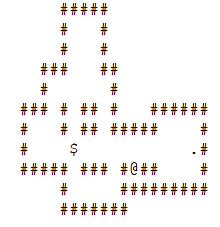
\includegraphics[width=5cm, height=5cm]{pic4.png}
		\caption{Game model}
	\end{figure}
	\section{Algorithms}
	Sokoban has many unique properties which are not there in other similar problems as Rubik’s cube or Lloyd Fifteen Puzzle. Moves are irreversible so making a bad move can make you lose the game. Given the game mechanics, several factors are taken into account for deciding on an optimal algorithm:
	(1) There is a need for returning a set of moves quickly because the game is played real time also. Consequently, an algorithm that is able to produce moves in a short amount of processing time and returns a strong move is desirable.
	(2) The constraint added to game. Constraints in this game refers to the walls that are present inside the outer boundary and restrict the path of the player.
	(3) The depth to which the search is constructed. Since this search problem can lead to multitudes of states and can at times lead to infinite search depths, once concern is to know how much the algorithm can explore in the search space. \br
	Given these considerations, we decided to evaluate considerable number of algorithms and compare them based on their space/time complexities. The strength of the algorithms in this space lies in their ability to quickly determine sequences of moves that yield relatively strong results. We have implemented four algorithms namely backtracking, Depth First Search (DFS), Breadth First Search (BFS) and Uniform Cost Search (UCS) and shown their results.
	\subsection{Baseline (\textit{Backtracking Algorithm)} and Oracle Implementation}
	The baseline of the project is the backtracking search algorithm and the oracle of the project is the high level human intelligence that is used to solve the game. So essentially, each level has a predefined number of moves which corresponds to the minimum moves that one can take to solve the game. This minimum number of steps forms the oracle. On the other hand, the backtracking algorithm is one of the simplest recursive algorithms and forms the baseline for our project but is seldom used widely because of its high time complexity. It just recurses to all states and finds the minimum cost in reaching the goal. The space complexity is O(D) and the time complexity is O($b^D$) which is very high. The implementation of Backtracking algorithm is as follows:
	\subsection{Depth First Search}
	Depth First Search (DFS) is a special case of backtracking search algorithm. The search starts from the root and proceeds to the farthest node before backtracking. The difference between this and the backtracking is that this stops the search once a goal is reached and does not care if it is not minimum. The space and time complexities, on the worst case, are the same as the baseline algorithm but stops when it finds the solution. The DFS algorithm is given below:
	\subsection{Breadth First Search}
	Breadth First Search (BFS), as the name says, explores the search space in the increasing order of the depth and the costs of traveling from one state to another is assumed to be a positive number. Typically, this algorithm is often associated with the concept of stack and queue and pushing and popping from the stack. Due to the larger states explored at shorter depths, the space complexity is very high of about O($b^d$) and the time complexity is O($b^d$). The pseudo code of BFS is:
	\subsection{Uniform cost Search}
	For any search problem, Uniform Cost Search (UCS) is the better algorithm than the previous ones. The search algorithm explores in branches with more or less same cost. This consist of a priority queue where the path from the root to the node is the stored element and the depth to a particular node acts as the priority. UCS assumes all the costs to be non negative. While the DFS algorithm gives maximum priority to maximum depth, this gives maximum priority to the minimum cumulative cost. It is implemented as:
	\section{Pruning Techniques}
	Pruning is a terminology used in machine learning and artificial intelligence that are used to reduce the size of the decision trees by removing the selected sections of the tree that provide undesirable results. We have implemented two techniques till now in the project and are described below:
	\subsection{Move appension}
	One of the primary problem in search problems is that the computation time becomes unimaginably high when the search space is big. In such cases, if we have priori knowledge about the systems, we can limit in the beginning of the search problem all the cases where we have impossible actions. For instance, the Figure 3 depicts a case where the only acceptable action is to move Up. The possible actions for any algorithm can be moving in all the directions which can be reduced to one by Move Appension where we restrict all the impossible actions. \br
	\begin{figure}[h!]
		\centering
		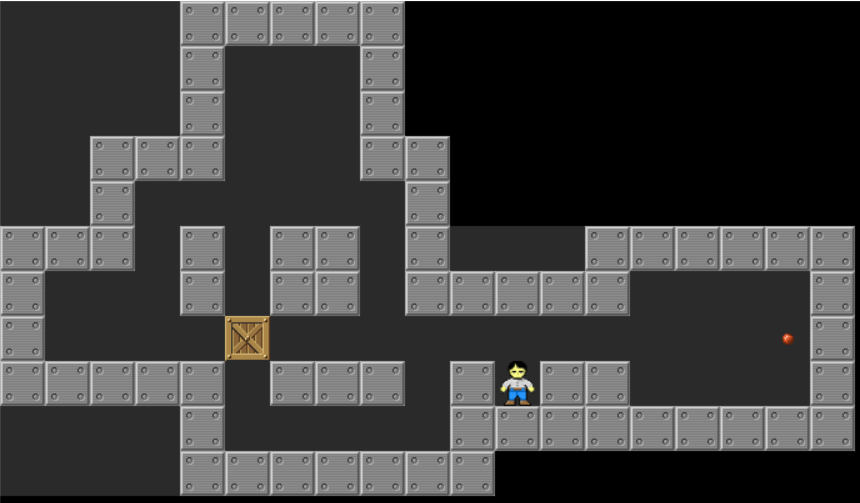
\includegraphics[width=6cm, height=5cm]{pic1.png}
		\caption{Move Appension Example}
	\end{figure}
	\subsection{Hashing}
	Hashing is a well known pruning method used to tune the algorithm to perform better. It follows the logic that decision which leads to the states that are already visited are considered as suboptimal. So all the states are stored in the hash table and at each point, a comparison is made between the current state and the stored state. If there is a match, the same action corresponding to the one in the hashing table is avoided.
	\section{Results}
	The performances of all the algorithm are calculated based on standard metrics like the time consumed, total number os states explored and the solution steps and are graphically represented in the Figures 4 and 5. The algorithms were implemented using two important characteristics. One was the time-out and the other was the Max-Depth. The algorithms were made to stop when it reached a certain predefined depth called the Max-Depth and is also terminated when it exceeded the maximum time, Time-out. This was necessary in order to prevent the algorithms from searching in infinite search space.\br
	It can be observed that the DFS exceeded the maxdepth and failed to perform in Levels 8,9 and 10. The time taken for it is significantly lesser than Backtracking but is greater than the other two algorithms. It was also observed that the states explored by all the algorithms were almost the same but they varied only by the time consumed and the solution steps.\br 
	There are two cost functions considered for UCS. The first cost function involves giving maximum cost to the action of pushing the crate out of target location followed by moving the crates followed by movement of the player. The second cost function was taken in a way where the first and third actions had equal cost. Naturally, it was observed that the second cost function of the UCS performed sluggishly than the first. \br \br \br \br
\begin{figure}[h!]
		\centering
	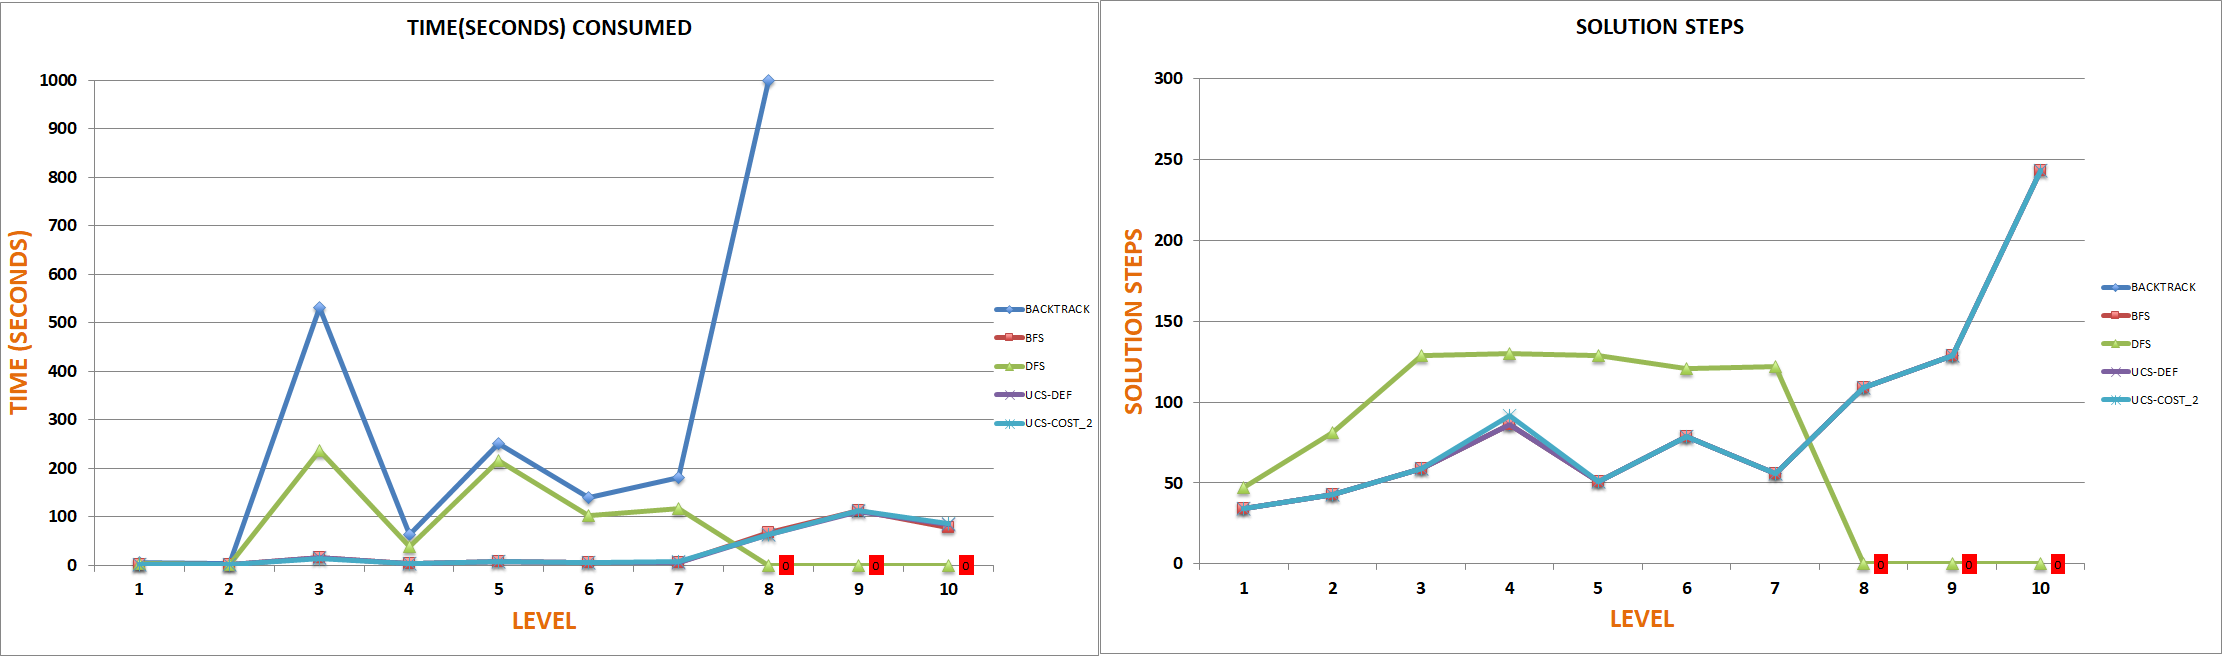
\includegraphics[width=18cm, height=6cm]{pic5.png}
	\caption{Time Consumed and Solution Steps}
\end{figure}
	\begin{figure}[h!]
	\centering
	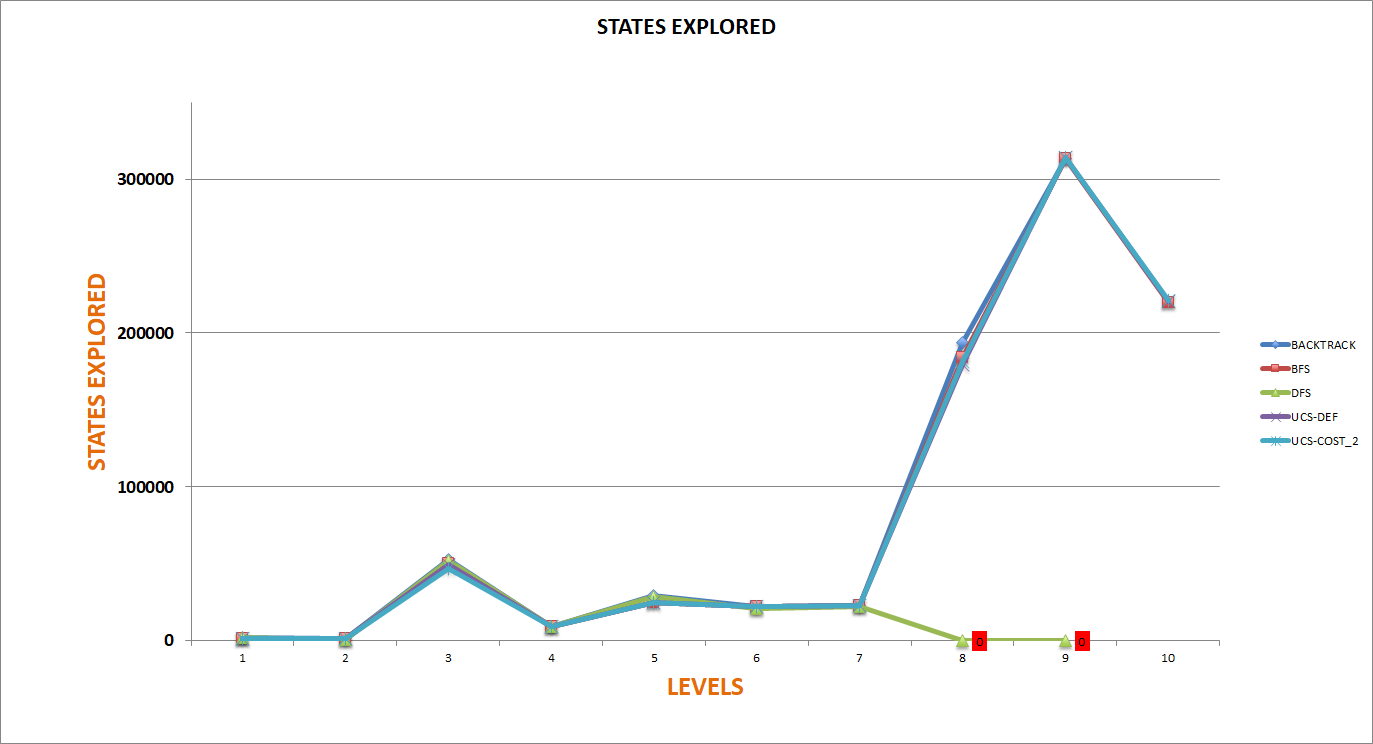
\includegraphics[width=9cm, height=6.5cm]{state_exp.png}
	\caption{States Explored}
\end{figure} \br
The algorithms for Backtracking, Depth First Search, Breadth First Search and Uniform Cost Search are given in the Appendix Section 1. The game play of the Sokoban game by the Uniform Cost Search Algorithm with the first cost function is implemented step by step and is provided in the Appendix Section 2.
	\section{Next Steps}
	We have implemented and extensively analyzed these four algorithms and compared based on their performances at different levels. Yet there are still other AI algorithms and pruning techniques which we would like to implement in the future. In particular, we plan to account for:
	\begin{itemize}
		\item implementing A* search algorithm with different heuristics. We are aiming to implement A* with Eucledian distance, Manhattan Distance and Hungarian Distance.
		\item exploring and trying to implement advanced search algorithms like the Depth First Search with Iterative Deepening (DFS-ID).
		\item learning and trying to implement more pruning techniques like the PI corral pruning, Dead lock Tables etc.
	\end{itemize}

	
	\newpage
	\section{Appendix 1 Algorithms}
	\begin{algorithm}\label{back}\small
	\caption{\small Backpropagation Algorithm$(state, maxdepth, maxtimeout)$}
	stack $\gets$ starting position of Sokoban \\
	\While{stack is not empty}{
		\eIf{Are crates on target}{put the state in option}{
			\eIf{Is deadlock or is depth $\ge$ maxdepth or is time $\ge$ maxtimeout}{pick next solution}{
				Get valid moves for Sokoban \\
				\ForEach{move}{
					Find next state \\
					Put it in stack	
			}}
	}}
	Pick the Best moves
\end{algorithm}

\begin{algorithm}\label{DFS}\small
	\caption{\small Depth First Search Algorithm$(state, maxdepth, maxtimeout)$}
	stack $\gets$ starting position of Sokoban \\
	\While{stack is not empty}{
		\eIf{Are crates on target}{break}{
			\eIf{Is deadlock or is depth $\ge$ maxdepth or is time $\ge$ maxtimeout}{pick next solution}{
				Get valid moves for Sokoban \\
				\ForEach{move}{
					Find next state \\
					Put it in stack	
			}}
	}} 
	return moves
\end{algorithm}

\begin{algorithm}\label{BFS}\small
	\caption{\small Breadth First Search Algorithm$(state, maxdepth, maxtimeout)$}
	queue $\gets$ starting position of Sokoban \\
	cost $\gets$ cost of moves \\
	\While{queue is not empty}{
		Remove the first element of queue
		\eIf{Are crates on target}{break}{
			\eIf{Is deadlock or is depth $\ge$ maxdepth or is time $\ge$ maxtimeout}{pick next solution}{
				Get valid moves for Sokoban \\
				\ForEach{move}{
					Find next state \\
					Put it in queue with current cost+1	
			}}
	}} 
	return moves
\end{algorithm}

\begin{algorithm}\label{UCS}\small
	\caption{\small Uniform Cost Search Algorithm$(state, maxdepth, maxtimeout)$}
	priority queue $\gets$ starting position of Sokoban \\
	cost $\gets$ cost of moves \\
	\While{queue is not empty}{
		Remove the highest priority element of queue
		\eIf{Are crates on target}{break}{
			\eIf{Is deadlock or is depth $\ge$ maxdepth or is time $\ge$ maxtimeout}{pick next solution}{
				Get valid moves for Sokoban \\
				\ForEach{move}{
					cost $\gets$ cost of move\\
					Add cost to current move
					Update queue with new cost and new state	
			}}
	}} 
	return moves
\end{algorithm}


\newpage
	\section{Appendix 2 Solution using UCS Algorithm}
		\begin{figure}[h!]
		%\centering
		{
			\begin{subfigure}[h!]{1.3in}
				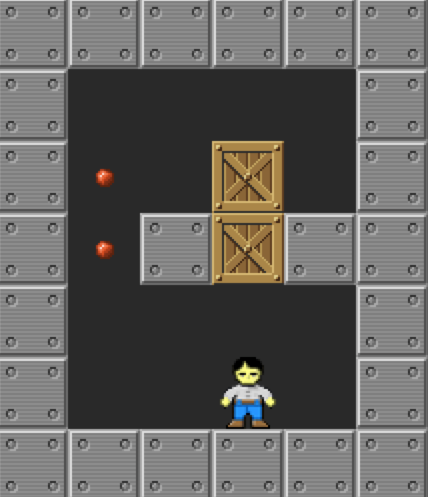
\includegraphics[height=1.5in]{p1.png}
			\end{subfigure}
		%	~$\mathbf{\Longrightarrow}$~
			\begin{subfigure}[h!]{1.3in}
				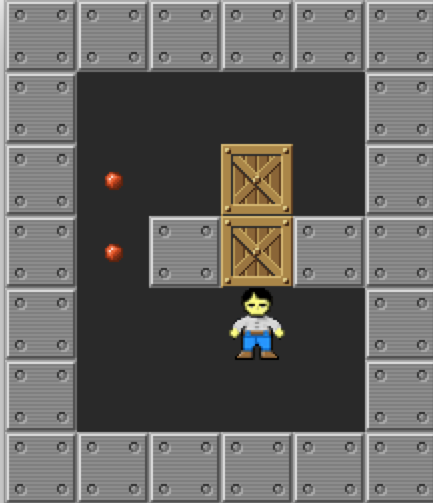
\includegraphics[height=1.5in]{p2.png}
			\end{subfigure}
		%	~$\mathbf{\Longrightarrow}$~
			\begin{subfigure}[h!]{1.3in}
				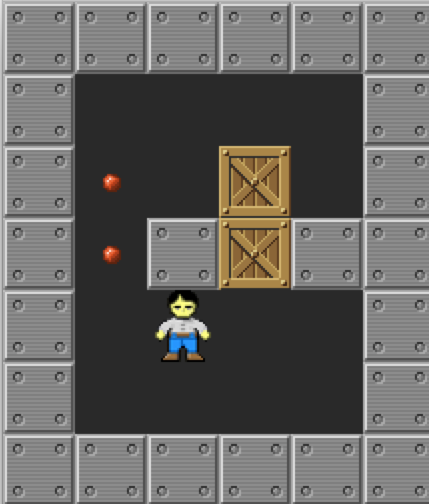
\includegraphics[height=1.5in]{p3.png}
		\end{subfigure}
		%~$\mathbf{\Longrightarrow}$~
	\begin{subfigure}[h!]{1.3in}
		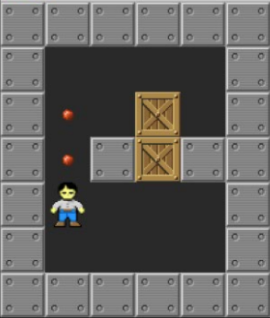
\includegraphics[height=1.5in]{p4.png}
\end{subfigure}
\begin{subfigure}[h!]{1.3in}
	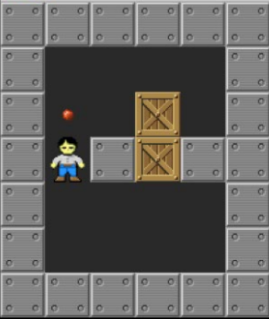
\includegraphics[height=1.5in]{p5.png}
\end{subfigure}}
		\label{fig:chain}
	\end{figure}

			\begin{figure}[h!]
		%\centering
		{
			\begin{subfigure}[h!]{1.3in}
				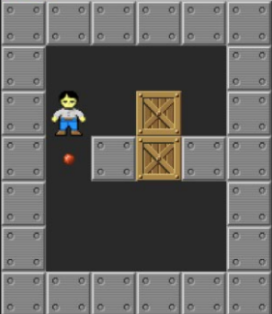
\includegraphics[height=1.5in]{p6.png}
			\end{subfigure}
			%	~$\mathbf{\Longrightarrow}$~
			\begin{subfigure}[h!]{1.3in}
				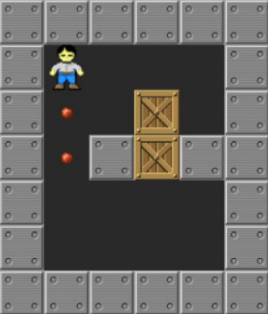
\includegraphics[height=1.5in]{p7.png}
			\end{subfigure}
			%	~$\mathbf{\Longrightarrow}$~
			\begin{subfigure}[h!]{1.3in}
				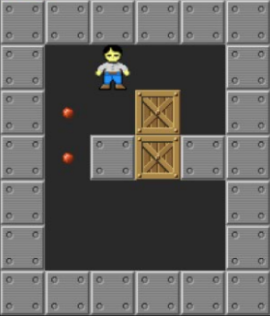
\includegraphics[height=1.5in]{p8.png}
			\end{subfigure}
			%~$\mathbf{\Longrightarrow}$~
			\begin{subfigure}[h!]{1.3in}
				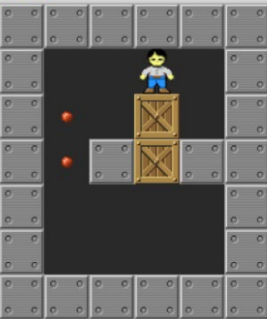
\includegraphics[height=1.5in]{p9.png}
			\end{subfigure}
			\begin{subfigure}[h!]{1.3in}
				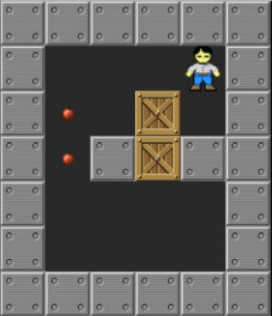
\includegraphics[height=1.5in]{p10.png}
		\end{subfigure}}
		\label{fig:chain}
	\end{figure}
				\begin{figure}[h!]
			%\centering
			{
				\begin{subfigure}[h!]{1.3in}
					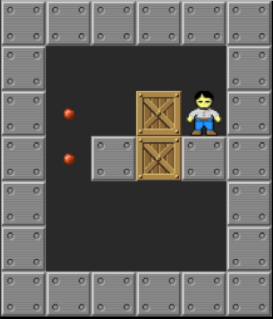
\includegraphics[height=1.5in]{q1.png}
				\end{subfigure}
				%	~$\mathbf{\Longrightarrow}$~
				\begin{subfigure}[h!]{1.3in}
					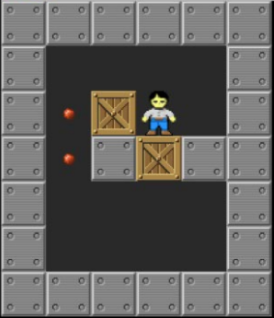
\includegraphics[height=1.5in]{q2.png}
				\end{subfigure}
				%	~$\mathbf{\Longrightarrow}$~
				\begin{subfigure}[h!]{1.3in}
					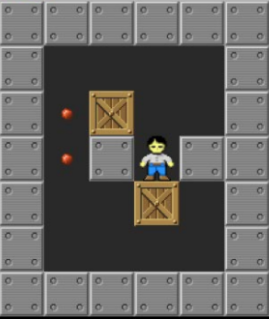
\includegraphics[height=1.5in]{q3.png}
				\end{subfigure}
				%~$\mathbf{\Longrightarrow}$~
				\begin{subfigure}[h!]{1.3in}
					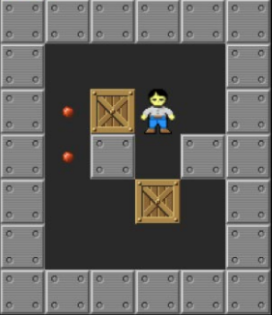
\includegraphics[height=1.5in]{q4.png}
				\end{subfigure}
				\begin{subfigure}[h!]{1.3in}
					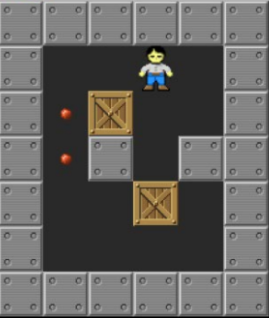
\includegraphics[height=1.5in]{q5.png}
			\end{subfigure}}
			\label{fig:chain}
		\end{figure}
		
		\begin{figure}[h!]
			%\centering
			{
				\begin{subfigure}[h!]{1.3in}
					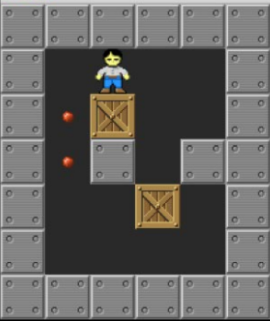
\includegraphics[height=1.5in]{q6.png}
				\end{subfigure}
				%	~$\mathbf{\Longrightarrow}$~
				\begin{subfigure}[h!]{1.3in}
					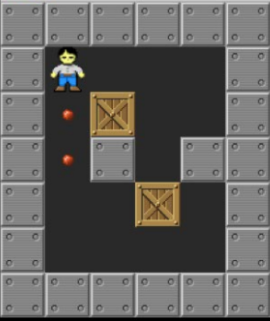
\includegraphics[height=1.5in]{q7.png}
				\end{subfigure}
				%	~$\mathbf{\Longrightarrow}$~
				\begin{subfigure}[h!]{1.3in}
					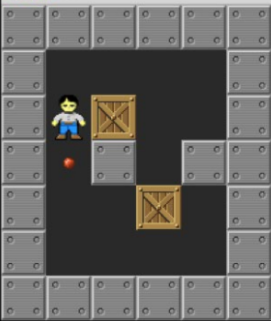
\includegraphics[height=1.5in]{q8.png}
				\end{subfigure}
				%~$\mathbf{\Longrightarrow}$~
				\begin{subfigure}[h!]{1.3in}
					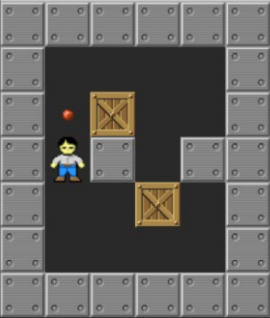
\includegraphics[height=1.5in]{q9.png}
				\end{subfigure}
				\begin{subfigure}[h!]{1.3in}
					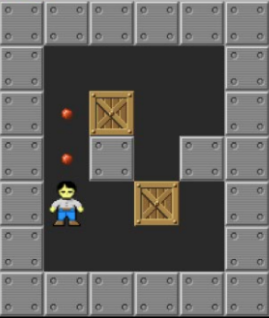
\includegraphics[height=1.5in]{q10.png}
			\end{subfigure}}
			\label{fig:chain}
		\end{figure}
				\begin{figure}[h!]
			%\centering
			{
				\begin{subfigure}[h!]{1.3in}
					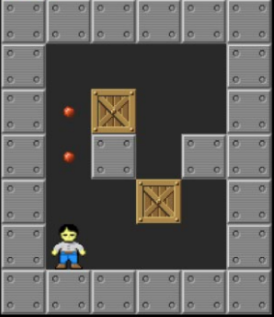
\includegraphics[height=1.5in]{r1.png}
				\end{subfigure}
				%	~$\mathbf{\Longrightarrow}$~
				\begin{subfigure}[h!]{1.3in}
					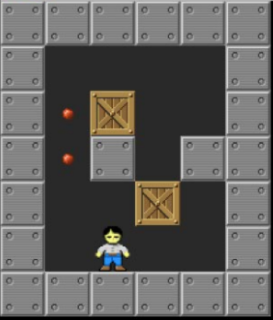
\includegraphics[height=1.5in]{r2.png}
				\end{subfigure}
				%	~$\mathbf{\Longrightarrow}$~
				\begin{subfigure}[h!]{1.3in}
					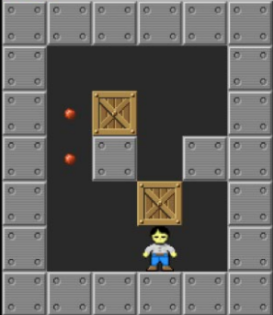
\includegraphics[height=1.5in]{r3.png}
				\end{subfigure}
				%~$\mathbf{\Longrightarrow}$~
				\begin{subfigure}[h!]{1.3in}
					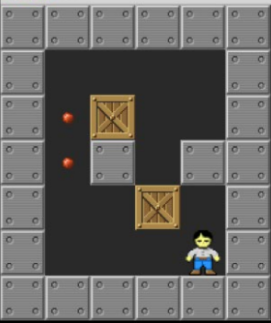
\includegraphics[height=1.5in]{r4.png}
				\end{subfigure}
				\begin{subfigure}[h!]{1.3in}
					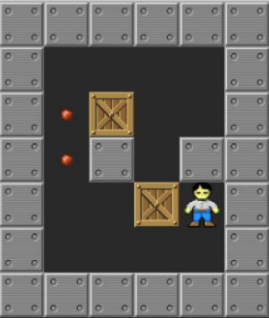
\includegraphics[height=1.5in]{r5.png}
			\end{subfigure}}
			\label{fig:chain}
		\end{figure}
		
		\begin{figure}[h!]
			%\centering
			{
				\begin{subfigure}[h!]{1.3in}
					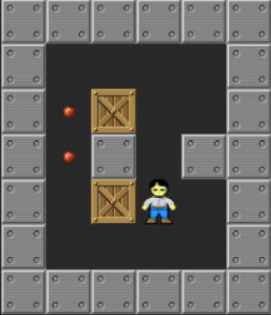
\includegraphics[height=1.5in]{r6.png}
				\end{subfigure}
				%	~$\mathbf{\Longrightarrow}$~
				\begin{subfigure}[h!]{1.3in}
					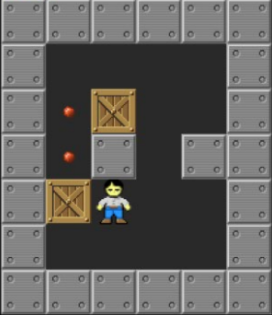
\includegraphics[height=1.5in]{r7.png}
				\end{subfigure}
				%	~$\mathbf{\Longrightarrow}$~
				\begin{subfigure}[h!]{1.3in}
					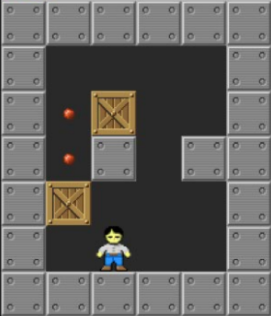
\includegraphics[height=1.5in]{r8.png}
				\end{subfigure}
				%~$\mathbf{\Longrightarrow}$~
				\begin{subfigure}[h!]{1.3in}
					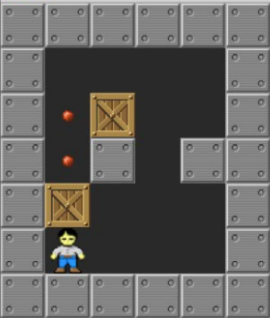
\includegraphics[height=1.5in]{r9.png}
				\end{subfigure}
				\begin{subfigure}[h!]{1.3in}
					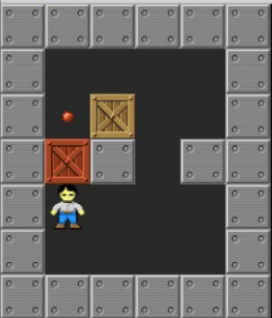
\includegraphics[height=1.5in]{r10.png}
			\end{subfigure}}
			\label{fig:chain}
		\end{figure}
						\begin{figure}[h!]
			%\centering
			{
				\begin{subfigure}[h!]{1.3in}
					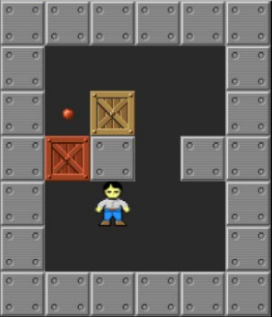
\includegraphics[height=1.5in]{s1.png}
				\end{subfigure}
				%	~$\mathbf{\Longrightarrow}$~
				\begin{subfigure}[h!]{1.3in}
					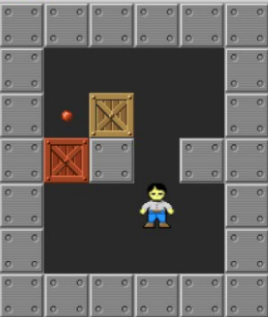
\includegraphics[height=1.5in]{s2.png}
				\end{subfigure}
				%	~$\mathbf{\Longrightarrow}$~
				\begin{subfigure}[h!]{1.3in}
					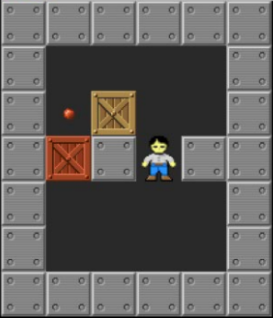
\includegraphics[height=1.5in]{s3.png}
				\end{subfigure}
				%~$\mathbf{\Longrightarrow}$~
				\begin{subfigure}[h!]{1.3in}
					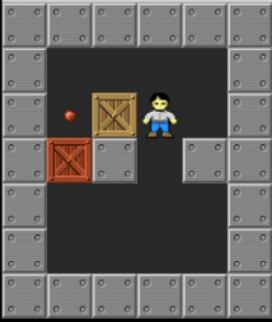
\includegraphics[height=1.5in]{s4.png}
				\end{subfigure}
				\begin{subfigure}[h!]{1.3in}
					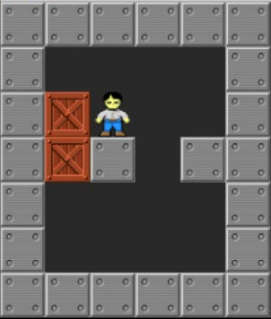
\includegraphics[height=1.5in]{s5.png}
			\end{subfigure}}
			\label{fig:chain}
		\end{figure}
	

\end{document}